%% LaTeX2e class for student theses
%% sections/content.tex
%% 
%% Karlsruhe Institute of Technology
%% Institute for Program Structures and Data Organization
%% Chair for Software Design and Quality (SDQ)
%%
%% Dr.-Ing. Erik Burger
%% burger@kit.edu
%%
%% Version 1.3.3, 2018-04-17

\chapter{Our Algorithm}
\label{ch:alg}

The algorithm and the underlying acceleration data structure we chose is inspired by the tree construction and traversal algorithm of the bounding volume hierarchy. Similarly to the BVH, we will construct a binary tree before rendering, and traverse through the tree to find the appropriate light when we are given the point of the intersection in the scene. Analogous to most BVH algorithms, our light BVH construction runs on a single thread, while the traversal can run on concurrent threads. Since the construction of the tree only a small fraction of the rendering time, this does not pose a problem even on scenes with over one million light sources.

\section{Informal Description of the Algorithm}
\label{sec:alg:idea}

In this section we will give rough overview of the ideas of our algorithm. We have thought about jumping straight into the in-depth implementation part and skipping the informal description of the algorithm but some parts of the implementation decisions are hard to understand without having at least a rudimentary overview of the algorithm. For instance, when we talk about the information every node of the tree needs to store, it is much easier for the reader to comprehend our train of thought when he has a general idea how our tree traversal algorithm works.

First, when we have access to all of the light sources of the scene, we want to create a binary tree data structure that includes every single light source of the scene. Similarly to the BVH construction, we will also split the scene spatially parallel to coordinate axis. We will also use a heuristic to find the best split of all three dimensions, comparable to the surface area heuristic. Our heuristic, the surface area orientation heuristic (SAOH) has some crucial difference to the SAH. First, instead of amounting the number of primitives, we will factor in the total emission power of the lights. Second, we have added an orientation factor. This orientation factor tries to keep light sources with similar orientations in the same node. This way, we have split the branches so different orientations most likely branch to different children of the tree and thus, finding the more likely child when traversing through the tree later will be clearer. When we have a node with only a single light source, this node is a leaf.

After we have constructed our tree, the next step would be traversing through the tree when we want to sample a light given an intersection point. Obviously, we don't just want to return a random light source which would make this algorithm pointless, but instead we want to importance sample a light that has most likely a strong contribution to the point. Therefore, we will define an importance measure for every node given the intersection point, that factors in the distance between the point and the node, the emission power of the node and an angle importance factor. We will start at the root of the tree and generate a uniform random number. Then, for every branch, a decision has to be made which child to take based on the importance measure and that random number. When we have arrived at a leaf node, that will be the light source we return.

What I have just described was our algorithm when we only want to sample a single light source. Conty and Kulla have shown in \cite{MLS}, that there are situations, where it is desirable to sample multiple light sources for one intersection point. That is the reason why we allow the user to define a split threshold. Based on the split threshold and a score which we calculate for every branch, instead of sampling only the left or the right child, we will sample both nodes. At the end, return one or multiple sampled lights. Afterwards, the sampled lights are used for the path tracing algorithm.

\section{Own Data Structures}
\label{sec:alg:ows}

In this section we will be discussing our own data structures. We will show our internal representation of our data structures now and reason why they are represented like this.

\subsection{Bounds\_o}

\begin{figure}
	\begin{center}
		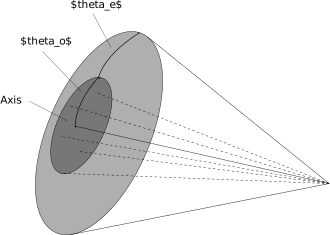
\includegraphics[width=0.3\textwidth]{bounds_o.png}
		\caption{Our internal representation of the Bounds\_o struct}
		\label{fig:boundso}
	\end{center}
\end{figure}

First we will introduce the Bounds\_o struct (\ref{fig:boundso}). This struct basically represents the orientation of a certain light source or a whole node. For a single light, the axis defines the orientation direction of the light source, while for a node, the axis represents the interpolated axes of all light sources included in the node. Theta\_o defines the minimum angle between the axis of the node and any light source included in this node. Theta\_e defines the additional emission range added to theta\_o for spotlights or area light sources. How we have pictured the geometric representation can be seen in \ref{fig:boundsogeo}. In our implementation, we accept point lights, spotlights and area light sources as light sources. This is how we initialize the Bounds\_o struct for single lights:

\begin{itemize}
	  \setlength\itemsep{0em}
	\item Point light
	\begin{itemize}
		  \setlength\itemsep{0em}
		\item Axis = (1, 0, 0)
		\item theta\_o = $\pi$
		\item theta\_e = $\pi/2$
	\end{itemize}
	\item Spot light
	\begin{itemize}
		  \setlength\itemsep{0em}
		\item Axis = spot direction
		\item theta\_o = 0
		\item theta\_e = spot's apperture
	\end{itemize}
	\item Area light
	\begin{itemize}
		  \setlength\itemsep{0em}
		\item Axis = normal of the geometric representation
		\item theta\_o = 0
		\item theta\_e = $\pi/2$
	\end{itemize}
\end{itemize}

\begin{figure}
	\begin{center}
		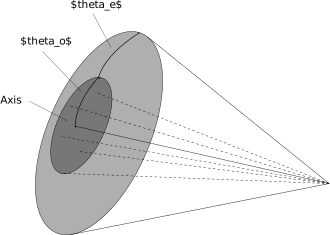
\includegraphics[width=0.6\textwidth]{bounds_o.pdf}
		\caption{geometric idea of the Bounds\_o struct}
		\label{fig:boundsogeo}
	\end{center}
\end{figure}

\subsection{Node representation}

We used two different implementations to represent a node in our light BVH tree (\ref{fig:lightbvhnode} and \ref{fig:linearlightbvhnode}). Both implementations are very similar, containing the two bounding bounds $bounds_w$ for the world space bounds and $bounds_o$ for the orientation bounds, as well as other other information that we will need for the tree traversal later. $Energy$ defines the combined energy of the lights under this node, $nLights$ describes the number of lights under this node, $centroid$ stores the centroid of the world space bounds, and $splitAxis$ stores the coordinate axis that splits the two children of this node. 

The main difference between the two implementations is the way to access the children of the nodes. In our $LightBVHNode$, we have explicit pointers to the two children, while we define the children implicitly in out $LinearLightBVHNode$. Since all of our $LinearLightBVHNodes$ are stored in aligned memory, the way we access the left child is just by incrementing the pointer of the current $LinearLightBVHNode$ by 1. The index needed to access the right child is stored in $secondChildOffset$. To access the second child, we just add $secondChildOffset$ to the base pointer of the root of the tree. If the node is a leaf of the tree and thus only contains one light source, $lightNum$ stores the index of that light source in both implementations.

\begin{figure}
	\begin{center}
		\includegraphics[width=0.5\textwidth]{lightbvhnode.png}
		\caption{Our internal representation of the LightBVHNode struct}
		\label{fig:lightbvhnode}
	\end{center}
\end{figure}

\begin{figure}
	\begin{center}
		\includegraphics[width=0.4\textwidth]{linearbvhnode.png}
		\caption{Our internal representation of the LinearLightBVHNode struct}
		\label{fig:linearlightbvhnode}
	\end{center}
\end{figure}



\section{Tree Construction}
\label{sec:alg:con}

In this section we will be talking about our in-depth implementation of the tree construction. The tree constructor method takes two parameters. First, a vector containing all the light sources in the scene. Second, we will take a parameter defining the split threshold that describes if we want to sample multiple light sources when traversing the light BVH later (\ref{subs:split}). The split threshold is a normalized value between 0.0 and 1.0. A split threshold of 1.0 never splits, we would only shade one light per point and a split threshold of 0.0 always splits, which means all lights of the scene are shaded. Note that our algorithm is implemented to work with any combination of point light sources, area light sources and spotlights.

\begin{algorithm}
	\caption{LightBVHAccelerator constructor}
	\label{LightBVHAccelerator}
	\begin{algorithmic}[1] % The number tells where the line numbering should start
		\Procedure{LightBVHAccel}{vector<light> lights, float splitThreshold}
		\State $LightBVHNode \; *root  \gets recursiveBuild(lights, 0, lights.size());$
		\State $LinearLightBVHNode \; *nodes \gets AllocAligned(totalNodes);$ 
		\State $flattenLightBVHTree(nodes, root, 0);$
		\EndProcedure
	\end{algorithmic}
\end{algorithm}

The $lightBVHAccel$ constructor initializes the tree construction. First, we will be using a recursive approach to build the light BVH. We will pass the light sources of the scene in an array and the starting and ending indices of the current node, obviously for the root of the light BVH we will pass the whole range of our vector. Then, after we have constructed our tree represented by $LightBVHNode$ objects, we will flatten the tree in a compacter form represented by $LinearLightBVHNode$ objects to ensure that our tree requires as little memory as possible and to improve cache locality. $Nodes$ will later be our object to run our tree traversal on.

\begin{algorithm}
	\caption{LightBVHAccelerator recursive build}
	\label{recursiveBuild}
	\begin{algorithmic}[1] % The number tells where the line numbering should start
		\Procedure{recursiveBuild}{vector<light> lights, int start, int end}
		\State LightBVHNode *node;
		\If{end - start == 1}
			\State *node = $initLeaf()$;
			\State \Return node;
		\EndIf
        \For{\texttt{every dimension}}
        	\State <calculate axis and thetas for the whole node for current dimension>
			\State <calculate all split costs for current dimension>
		\EndFor
		\State <find out best split>
		\State *node = $initInterior(recursiveBuild(leftChild), recursiveBuild(rightChild));$ \\
		\Return node;
		\EndProcedure
	\end{algorithmic}
\end{algorithm}

Our implementation of the light BVH construction can be split into multiple sections. Obviously, first, we want to cover the base case, when we only have a single light source under the node. In this case, we cannot split further, so we will just initialize a leaf node with the one light source and return this leaf node.


\section{Tree Traversal}
\label{sec:alg:tra}

\subsection{Splitting}
\label{subs:split}